\documentclass[11pt]{beamer}
\usetheme{Dresden}
\usecolortheme{beaver}
%\usetheme{CambridgeUS}
\usepackage[utf8]{inputenc}
\usepackage[ngerman]{babel}
\usepackage[T1]{fontenc}
\usepackage{graphicx}
\usepackage{listings}
%\usepackage{schule}
\author{van Heteren-Frese}
\title{in-z2}
\subtitle{}
%\logo{} 
\institute{Schadow Gymnasium} 
%\date{} 
%\subject{} 

\AtBeginSection[]{
\frame{
\frametitle{Inhaltsverzeichnis}
\tableofcontents[currentsection]
}
}
\renewcommand{\arraystretch}{0}
\begin{document}
\begin{frame}{Verschlüsseln ohne Austausch geheimer Informationen}
Auch bei unknackbaren Verschlüsselungsverfahren besteht stets die Gefahr, dass jemand das geheime Schlüsselwort erfährt. Bevor Nachrichten verschlüsselt werden können, müssen sich die Kommunikationspartner stets auf einen gemeinsamen Schlüssel einigen. Deshalb haben in der zweiten Hälfte des 20. Jahrhunderts einige Wissenschaftler erforscht, ob es nicht ein Verfahren geben kann, bei dem keine geheimen Schlüssel ausgetauscht werden müssen.
\end{frame}
%
\begin{frame}{Szenario}
\small
Stellen Sie sich folgende Situation vor: Alice und Bob haben \alert{je ein Schloss mit Schlüssel}.
Alice möchte Bob ein Geheimnis in einer verschlossenen Kiste übermitteln.
\begin{block}{Fragestellung:}
	Wie kann Alice den Inhalt der Kiste sicher übermitteln, ohne Bob den Schlüssel für ihr Schloss zu geben?
\end{block}
\end{frame}
%
\begin{frame}{Aufgabe: Sichere Übertragungsmethode finden}
\begin{itemize}
\item Schreiben Sie eine Nachricht an Ihre Partnergruppe. \glqq Verschlüsseln\grqq\  Sie die Nachricht mit Hilfe eines Umschlages und eines Schlosses.
\item Übermitteln Sie die Nachricht an den Postboten, der sie dem Empfänger zustellt.
\item \textbf{Ziel:} Der Postbote darf die Nachricht nicht mitlesen. Trotzdem muss der Empfänger die Nachricht entschlüsseln können!
\end{itemize}
\end{frame}

\begin{frame}{Regeln}
\begin{enumerate}
\item Sie müssen:
\begin{itemize}
\item Die verschlüsselte Nachricht dem \glqq Postboten\grqq\ übergeben. Dieser liefert die Nachricht aus.
\end{itemize}
\item Sie dürfen:
\begin{itemize}
\item Sich vorab persönlich treffen
\end{itemize}
\item Sie dürfen \textbf{nicht:}
\begin{itemize}
\item Die Nachricht persönlich übergeben. (Persönliche treffen dienen nur dem Austausch über das anzuwendende Verfahren)
\end{itemize}
\end{enumerate}
\begin{center}
\begin{tabular}{ccc}
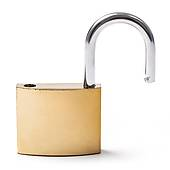
\includegraphics[width=2.1cm,clip,trim=0cm .4cm 0cm 0cm]{schloss} & 
%\hspace*{.5cm}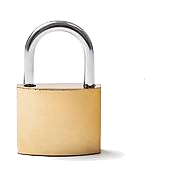
\includegraphics[width=2.5cm,clip,trim=0cm .4cm 0cm 0cm]{schloss_2}&

\includegraphics[width=2.1cm]{umschlag}&
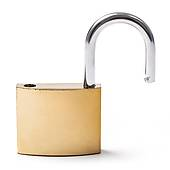
\includegraphics[width=2.1cm,clip,trim=0cm .4cm 0cm 0cm]{schloss} \\
\hspace*{-.7cm}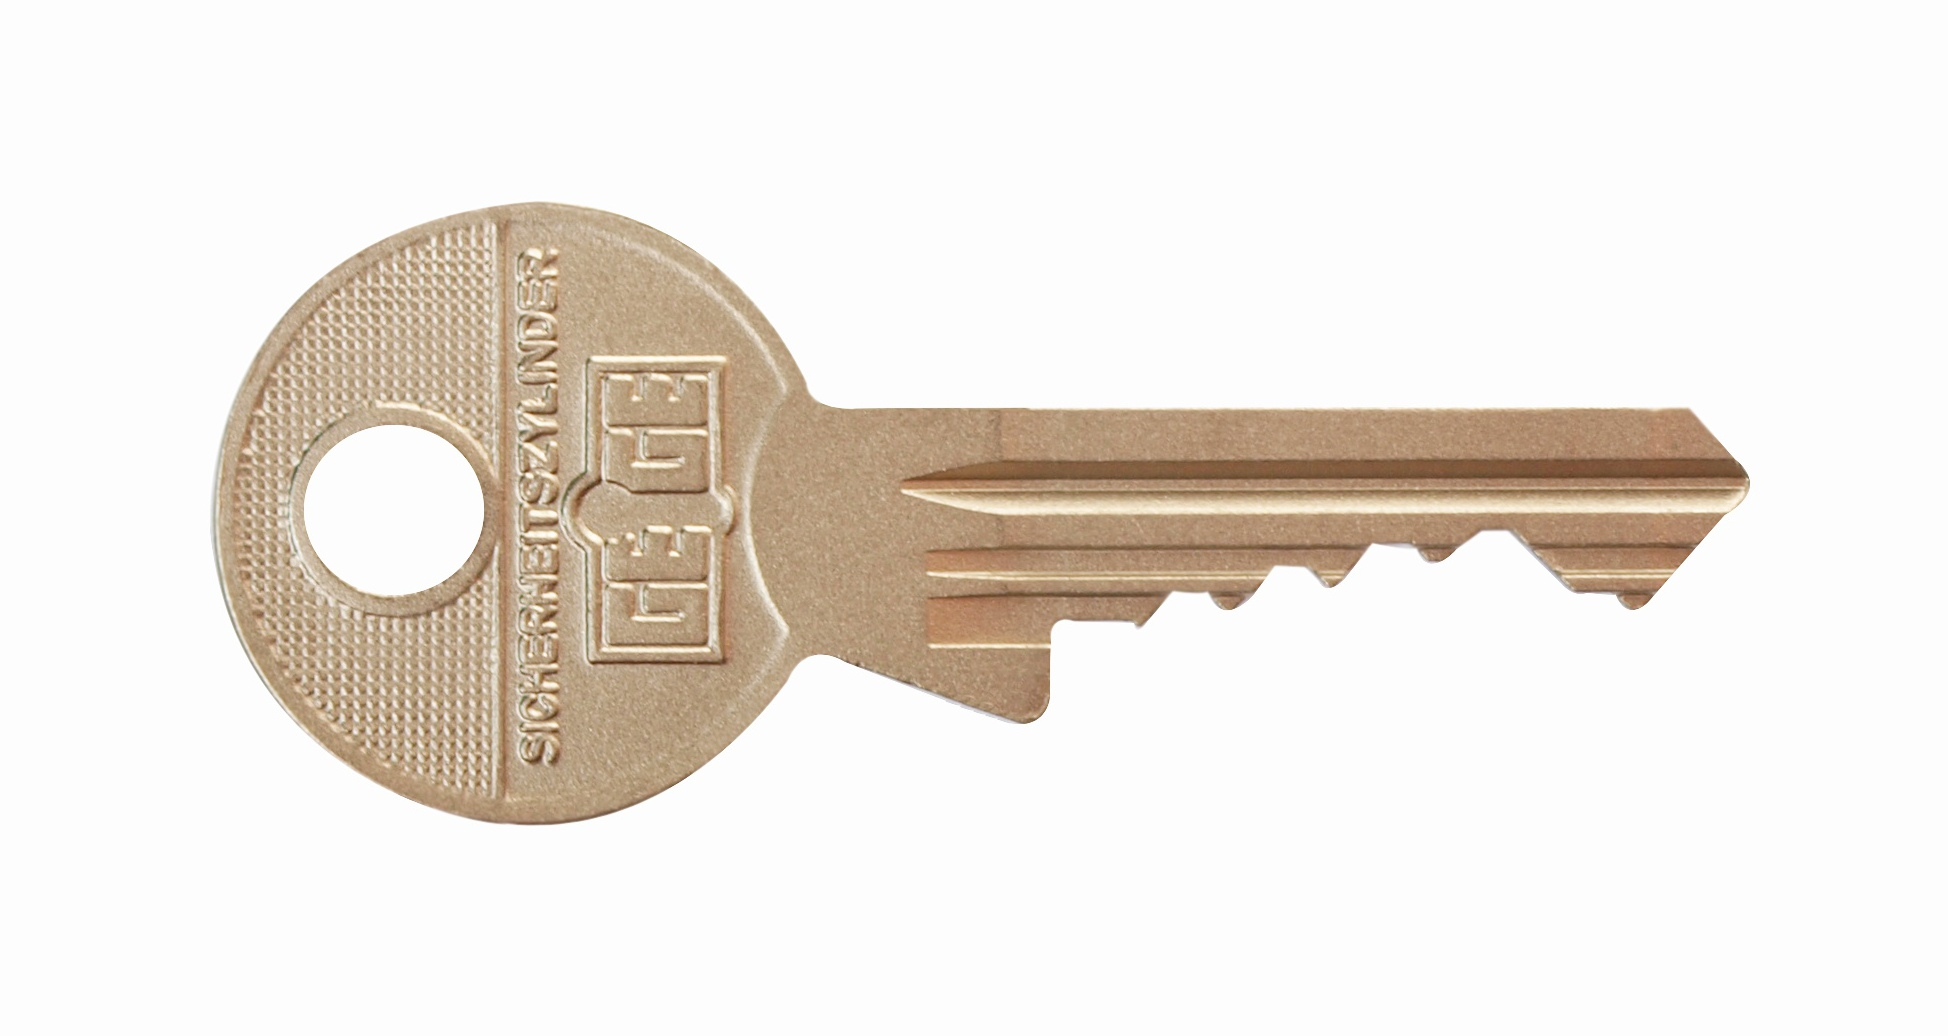
\includegraphics[angle=90,width=.8cm,clip,trim=1cm 2cm 30cm 2cm]{key}& &
\hspace*{-.7cm}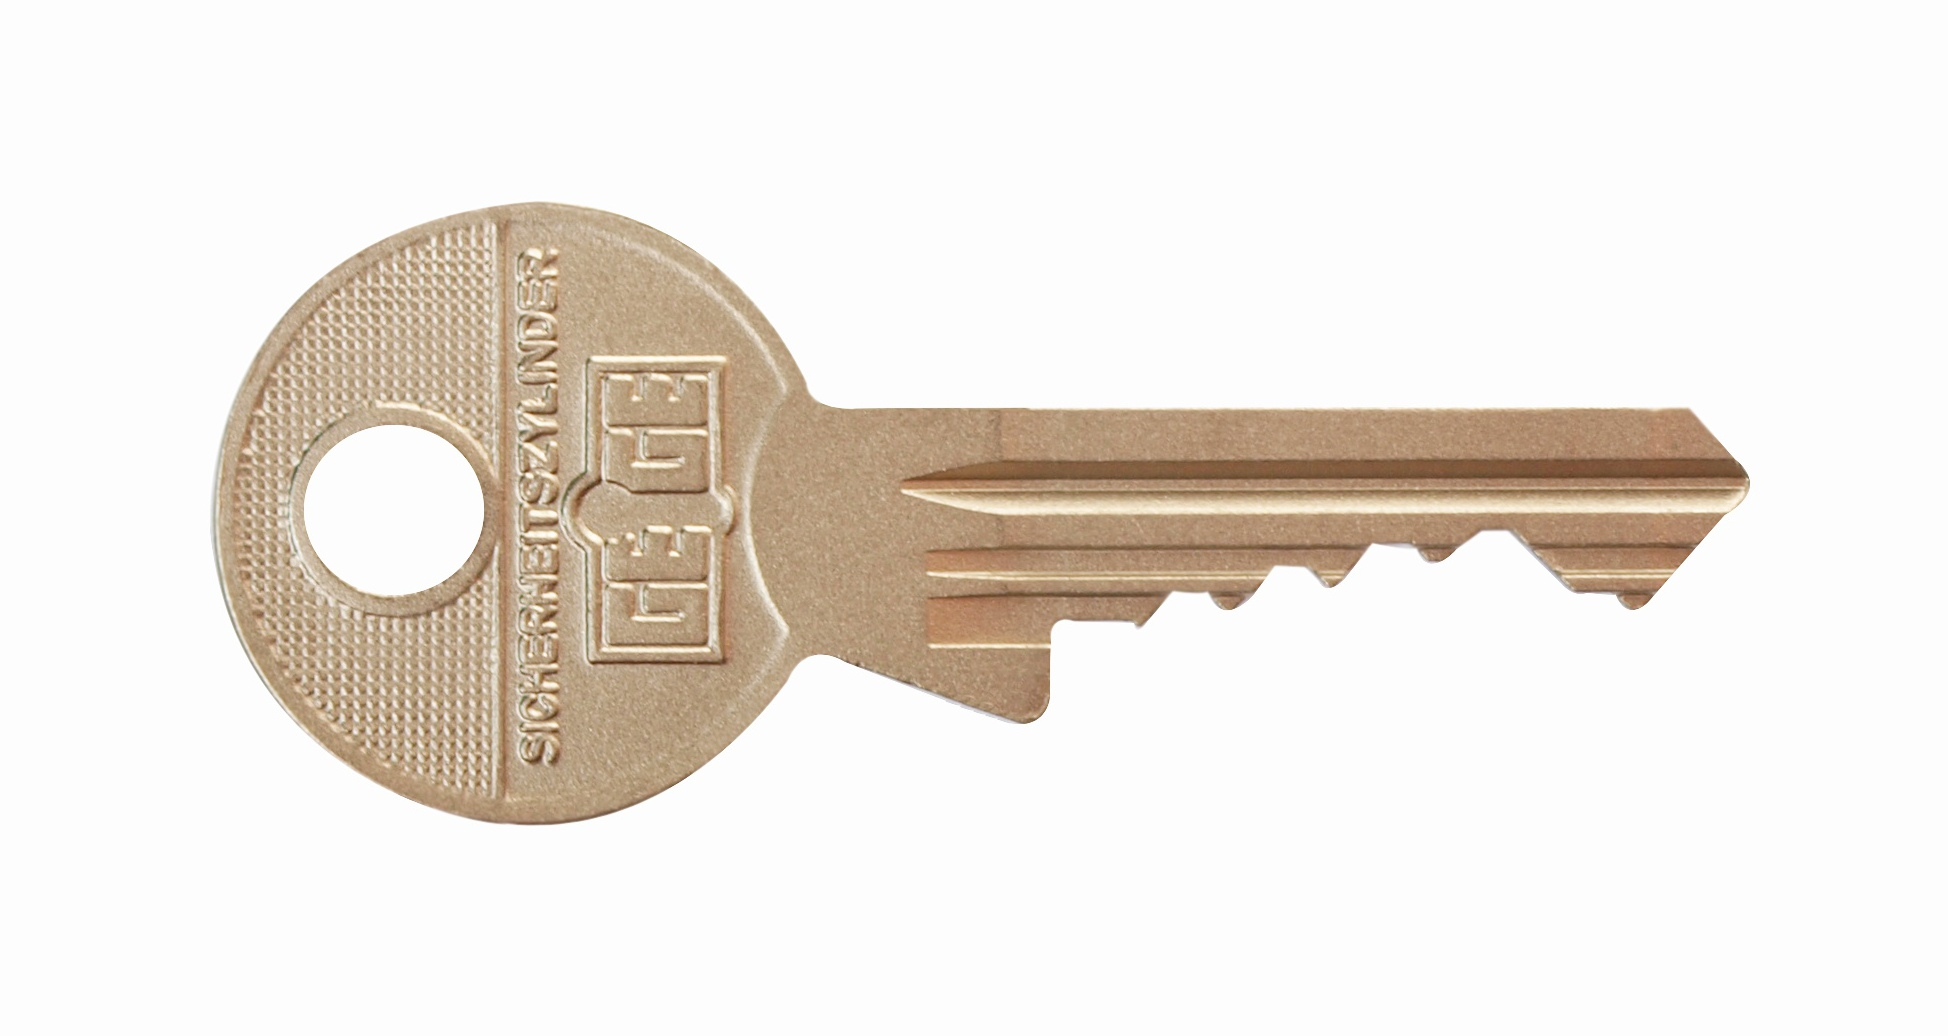
\includegraphics[angle=90,width=.8cm,clip,trim=1cm 2cm 30cm 2cm]{key}
\end{tabular}
\end{center}
\end{frame}


\end{document}